%%%%%%%%%%%%%%%%%%%%%%%%%%%%%%%%%%%%%%%%%%%%%%%%%%%%
\section{Informed Plan Selection}\label{sec:coverage}
%%%%%%%%%%%%%%%%%%%%%%%%%%%%%%%%%%%%%%%%%%%%%%%%%%%%

In this section, we extend our BDI learning so as to include a confidence test
within the plan selection mechanism itself. More concretely, in the new approach,
instead of using the stability measure to ensure that we only record results that
we are confident in, we instead modify our plan selection procedure to take into
account of how confident we are in the current decision tree.
% %
The idea is simple: the confidence on a plan's decision tree increases as the
different possible choices below the plan (in the goal-plan structure) are better
explored.
% %
Note that while the stability mechanism ensures that failure information is
\emph{not recorded} against a decision tree until the corresponding goal-plan
structure is adequately explored; the new approach instead influences how the
decision tree is \emph{use} at plan selection time.


So, with each plan in the goal-plan tree hierarchy, we identify its set of
potential \textit{choices} as the set of all potential execution paths
\textit{below} the plan in the hierarchy. Observe this can easily be computed
offline beforehand.
% %
Roughly speaking, a plan's decision tree is more \textit{informed} for a world
state, if it accounts for a larger number of plan's choices in that state.
% %
Next, we say that a plan has a higher degree of \emph{coverage} when more of its
underlying choices have been explored in the past and accounted in the
corresponding decision tree.
% %
Technically, given a decision tree $T$ for given plan, we define its converge
$c_T(w) \in [0,\ldots,1]$ as the coverage degree of $T$ for world state $w$.
% %
Initially, when the plan has not yet been executed in a world $w$, its coverage
on the state, namely $c_T(w)$, is zero and the agent may not be that confident on
the probability of plan success estimated by the decision tree at $w$. As the
different ways of execution the plan in the world are explored, the value of
$c_T(w)$ approaches $1$. When all choices have been tried, $c_T(w)=1$ and the
agent may rely on the decision tree estimation of success fully.
% %
Put differently, the coverage degree provides a confidence test on the decision
tree.




Next,	 one can define an equation for determining the final plan selection
weight for a plan that is influenced by the above coverage-based confidence measure.
% %
Formally, we define the plan's weight for plan selection, namely $\Omega'(w)$, based
on the plan success expectation returned by the decision tree and the current
coverage degree:
%
\begin{equation*}\label{eqn:coverage}   
\Omega_T(w) = 0.5 + \left[  c_T(w) *  \left( p_T(w) - 0.5 \right)  \right].
\end{equation*}
	
	
Initially, the weight of the plan for a world where it has never been executed is
assigned a default value ($0.5$ in our case).
% %
As the coverage degree increases with time, by trying the various ways the plan
could be executed, the weight of the plan approaches the true value estimated by
the plan's decision tree.



Regarding how the coverage degree is calculated at every point, we should make
the following two observations.
% %
First, the coverage $c_T(w)$ for a world $w$ is calculated and stored each time a
result is recorded against a plan's decision tree $T$.
% %
Second, it requires, in principle, $\tau \times |S|$ \emph{unique} executions of
a plan for it to reach \emph{full} coverage, where $\chi$ is the total number of
choices below the plan and $|S|$ is the number of possible worlds. Practically,
however, it takes significantly less since choices below a plan are effectively
represented by an AND/OR tree, and each time an AND node fails, the subsequent
nodes are not tried and are accounted covered for the world in question.
% %
Moreover, since plans are typically executed in the context of other plans
(e.g., the plan to check-in is always executed after a plan to go to the
aiport), it would not be necessary to account for the whole world space, but
only for its subset that is relevant for the plan.

\newcommand{\CLSELA}{\mbox{$\CL\!\!+\!\!\Omega$}}
\newcommand{\CLSELB}{\mbox{$\CL\!\!+\!\!\Omega'$}}
\newcommand{\BULSELA}{\mbox{$\CL\!\!+\!\!\Omega$}}
\newcommand{\BULSELB}{\mbox{$\CL\!\!+\!\!\Omega'$}}

\medskip With the new account for plans' weight, we (re)considered the two
learning approaches \CL\ and \BUL\ from the previous section with a plan
selection based on such weights. We shall refer to such new agents as \CLSELB\
and \BULSELB, respectively.
% %
Similarly, let us call $\CLSELA$ and $\BULSELA$ the corresponding agents using
the \emph{original} probabilistic selection where the weight of a plan depends
only on its decision tree success expectation $\Omega_T(w) = p_T(w)$.



In Figure~\ref{fig:performance-applicability}, we show the performance of all
four BDI learning agents in structures $\T_2$ and $\T_4$.
% %
First of all, when it comes to the \BUL\ stabibility-based learning scheme, the
two variations, namely $\BULSELA$ and $\BULSELB$, always show similar
performance.
% %
This is not surprising, as the stability test performed by these agents at each
plan node inherently results in close to full coverage of the plan, thus
effectively reducing $\Omega'_T(w)$ to $\Omega_T(w)$.

\textbf{********* Sebastian: I am at this point ***********}


For the \CL-favouring structure $\T_1$ we find that the new \CL+$E'$
configuration performs equally well to the original \CL+$E$
configuration, so while there is no significant improvement there is
also no loss in performance. Similarly, for the balanced structure
$\T_3$ where both \CL\ and \BUL\ perform equally well, the \CL+$E'$
configuration shows no significant improvement. For $\T_1$ and $\T_3$
then, the $+E'$ results are the same as those reported for the
original $+E$ configurations in Figure \ref{fig:T1_result} and Figure
\ref{fig:T3_result}. 

The impact of $E'$ is apparent in $\T_2$ however, a structure that
favours the conservative \BUL\ approach (Figure
\ref{fig:T2_result}). Here \CL+$E'$ shows a dramatic improvement over
\CL+$E$. Figure \ref{fig:T2_result2} shows this change with the new
$+E'$ configurations (diamonds for \BUL\ and squares for \CL)
superimposed over the original $+E$ results of Figure
\ref{fig:T2_result} (circles for \BUL\ and triangles for \CL). So for
the \BUL-favouring structure $\T_2$, the \CL+$E'$ (squares) approach
is now much closer to \BUL\ performance than the previous \CL+$E$
(triangles) approach. 


\begin{figure*}[t]
\begin{center}
\subfigure[Structure $\T_2$]{\label{fig:T2_result2}
%!TEX root = ../dsingh-aamas10-poster.tex
\begin{tikzpicture}[x= 0.00533cm,y=9cm]
	\definecolor{darkblue}{rgb}{0.1,0.1,0.5}
	\definecolor{darkred}{rgb}{0.8,0.0,0.1}
    % Draw the axes and grid lines
    \draw[-] (0,0) -- (0,1) -- (3000,1) -- (3000,0) -- cycle; 
    \draw[-,thin, dotted, ystep=0.2, xstep=3000] (0,0) grid (3000,1);
    \foreach \x in {500, 1500, 2500}  \draw [-,xshift=0](\x,4pt) -- (\x,-1pt);
    \foreach \y in {0.0,0.2,0.4,0.6,0.8,1.0}  \draw [-,yshift=0](4pt,\y) -- (-1pt,\y);
    \foreach \x/\xtext in {500/500, 1500/1500, 2500/2500} \node at (\x,0) [below] {\xtext};
    \foreach \y/\ytext in {0.0,0.2,0.4,0.6,0.8,1.0}  \node at (0,\y) [left] {\ytext};
    \node at (0,1.15) {Success};
    \node at (2500,0.1) {Iterations};
    \draw[-,darkred] plot[mark=x,mark size=10,mark options={color=darkred}] 
			file {figs/data/test05v3gm.CC.tikzdata};
    \draw[-,thin, densely dashed,black] plot[mark=x,mark size=10,mark options={color=black}] 
			file {figs/data/test05v3gm.CP.tikzdata};
    \draw[-,darkblue] plot[mark=o,mark size=6,mark options={color=darkblue}] 
			file {figs/data/test05v3gm.SP.tikzdata};
    % Also draw the expected convergence: 0.9^8 actions=0.43046
    \draw[dashed,-,yshift=0](0,0.43046) -- (3000,0.43046);
	\node at (3450,0.5) {$\mathcal{T}2$};

\end{tikzpicture}

}
\qquad
\subfigure[Structure $\T_4$]{\label{fig:T4_result}
%!TEX root = ../dsingh-aamas10.tex
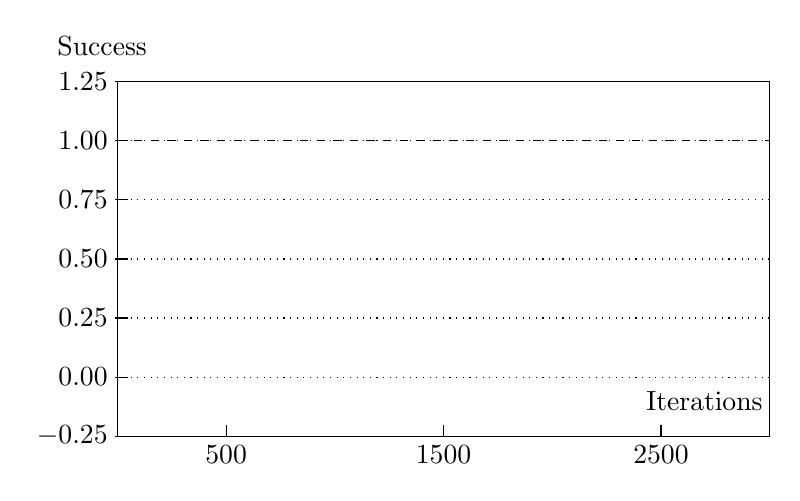
\begin{tikzpicture}[x=0.00276cm,y=3cm]
    % Draw the axes and grid lines
    \draw[-] (0,-0.25) -- (0,1.25) -- (3000,1.25) -- (3000,-0.25) -- cycle; 
    \draw[-,thin, dotted, ystep=0.25, xstep=3000] (0,-0.25) grid (3000,1.25);
    \foreach \x in {500, 1500, 2500}  \draw [-,xshift=0,yshift=-0.25](\x,-0.20) -- (\x,-0.25);
    \foreach \y in {-0.25,0.00,0.25,0.50,0.75,1.00,1.25}  \draw [-,yshift=0](4pt,\y) -- (-1pt,\y);
    \foreach \x/\xtext in {500/500, 1500/1500, 2500/2500} \node at (\x,-0.25) [below] {$\xtext$};
    \foreach \y/\ytext in {-0.25,0.00,0.25,0.50,0.75,1.00,1.25}  \node at (0,\y) [left] {$\ytext$};
    \node at (-70,1.4) {Success};
    \node at (2700,-0.1) {Iterations};
    \draw[-,red] plot[mark=x,mark size=4,mark options={color=red}] 
			file {figs/data/test05v3gmt.CP.tikzdata};
    \draw[-,blue] plot[mark=o,mark size=2,mark options={color=blue}] 
			file {figs/data/test05v3gmt.SP.tikzdata};
    % Also draw the expected convergence: 0.9^8 actions=0.43046
    \draw[dashed,-,yshift=0](0,1.0) -- (3000,1.0);

\end{tikzpicture}

}

\caption{Comparison of the new configurations \BUL+$E'$ (diamonds) and \CL+$E'$
(squares) against the earlier \BUL+$E$ (circles) and \CL+$E$ (triangles) for the
\BUL-favouring structure $\T_2$.}
\end{center}
\end{figure*}


We now consider a new structure $\T_4$ that is based on the typical setting (so
is not intentionally biased towards one approach), and that has the property that
a world $W$ may have two solutions, each in a different sub-tree. Furthermore one
solution is always \textit{better} than the other because it has a higher chance
of success (in our environment we model this by varying the number of actions
required in the solution where each action has a $10\%$ chance of failure).
Finally, the structure is crafted so that the likelihood of finding the
sub-optimal solution is higher. The purpose is to understand how our approaches
behave when optimality is important. Here we expect that the coverage-based
exploration of $E'$ should benefit over $E$ in finding the optimal solutions
first.


Figure \ref{fig:T4_result} shows the results for $\T_4$ where \CL+$E'$ (squares)
easily outperforms \CL+$E$ (triangles) and \BUL (diamonds and circles). The
reason why the other configurations are sub-optimal is because they do not take
into account the structure of the tree and therefore tend to focus exploration in
the sub-tree where the first solution was found (which likely is the sub-optimal
one in our case) \footnote{Note that \BUL+$E'$ does consider the tree structure
but as explained earlier it's behaviour is effectively the same as \BUL+$E$}.


The above results are significant because they highlight a configuration \CL+$E'$ that performs well in \textit{all} proposed structures: the \CL-favouring $\T_1$, the \BUL-favouring $\T_2$, the typical setting $\T_3$, and the typical setting with optimal solutions $\T_4$, making it a good candidate for the general setting. Moreover, the \CL-based configuration is a simpler alternative to the \BUL-based configuration, further adding to it's appeal.

\Omit{
\subsection{Discussion}

In Section \ref{sec:coverage} we presented a \textit{coverage}-based
confidence measure that combined with the \dt classification gives an
informed plan selection function (Equation \ref{eqn:coverage}) that
benefits our context learning approaches \CL\ and \BUL. Now, 
}
Since the
coverage $c_T(S)$ in Equation \ref{eqn:coverage} is simply a
confidence measure, then the way it is \textit{used} will determine
the weighting of the confidence in the final plan selection
probability $p'_T(w)$. For instance we could replace $c_T(S)$ in
Equation \ref{eqn:coverage} with $c_T(S)^{1/b}$ where $b$ is the
weighting (and $b=1$ gives us the original Equation
\ref{eqn:coverage}). Then adjusting $b \rightarrow 0, (0 \ne b < 1$)
we get more \BUL+$E$-like performance, while adjusting $b \rightarrow
\infty (b > 1)$ will result in more \CL+$E$-like performance. In fact,
an improved agent could reference the (static) goal-plan tree
structure at runtime and adjust $b$ automatically based on the offline
compiled knowledge of which approach works better for which tree
topology. 
% This extension is left as a future implementation exercise. 

We noted earlier in Section \ref{sec:experiments} that plan execution
in real systems is often not cost-free, so presumably the agent would
not execute a plan with too low a probability of success. We also show
that such deliberation does not favour \CL\ but does \BUL. It is clear
that choosing not to execute a plan below a threshold probability of
failure would also hurt the \CL+$E'$ configuration (though
not as much as \CL+$E$). For such systems, we suggest that the
weighting $b$ be used to get the preferred \BUL-like performance. 

One critique of the coverage-based confidence measure is that it has a
defined start ($c_T(S)=0$) and end state ($c_T(S)=1$). For a real
system however, learning and re-learning will occur in an endless loop
as the agent continually tries to adapt to a changing
environment. This implies that our confidence in a \dt's
classification would also require calibration based on a changing
environment. If the change in the environment is deliberate (for
instance the agent was moved into a new environment) then the coverage
$c_T(S)$ could be reset and confidence \textit{re-built}. Without such
a signal the agent must rely on measuring per-goal performance in
order to pick up failures that could be attributed to environmental
changes. The problem of identifying changes that warrant new learning
as compared to adapting previous learning, however, is generally
considered to be very difficult.
%a much harder one. 

